% Part 2 §2.11. Carries "Quantum Darwinism at Cosmological Scales" (Mar 2026), "Gravitational Decoherence from Dual-Sector Thermodynamics" (Feb 2026)
% and "Entanglement, Decoherence, and the Thermodynamic Cost of Classical Records" (Oct 2026 rev.), all read in full 2026-10-02 (861, 478, 253 lines).
% Numbers: docs/verification/scripts/verify_quantum_darwinism.py, verify_bottom_up_exponent.py, verify_grav_decoherence.py.
% Checks: docs/verification/quantum/*_CHECK.md, docs/verification/theory/BOTTOM_UP_EXPONENT.md. Measurement and time: Part 5.
\chapter{Records at the quantum scale}\label{ch:quantumrecords}

\section*{The place}
IAM's Law (Chapter~\ref{ch:iams_law}): every irreversible transition from a quantum superposition to a classical record pays at least $k_BT\ln2$ per bit,
at the temperature of the surface where the record is written. Earlier chapters followed the law outward to the cosmic horizon. This chapter follows it
down to where records begin --- the quantum-to-classical transition itself --- and back up again, to show that the cosmic ledger $E(a)$ is the sum of
those transitions.

\section{What decoherence explains, and what it leaves open}
A system $S$ interacting with an environment $\mathcal E$ evolves unitarily into $\sum_i c_i|s_i\rangle|e_i\rangle$. Tracing out the environment
suppresses the off-diagonal terms; the states that survive monitoring are the pointer states (einselection; Zurek 1981, 2003~\cite{Zurek1981,Zurek2003}). Quantum Darwinism adds
objectivity: information about the pointer state is copied redundantly into many independent fragments of the environment, so that many observers can
read the same outcome without disturbing it (Zurek 2009~\cite{Zurek2009}). Decoherence theory explains how classical records form and why they agree. It does not say
what a record costs, or where it is ultimately kept.

IAM's Law answers both. Each irreversible record costs $k_BT\ln2$ per bit, paid at the nearest encoding surface. A record in a detector is paid at the
detector; a record made by a collapsing cloud of matter is paid at the largest surface that matter shares, the cosmic horizon at
$T_{GH}=\hbar H/2\pi k_B$. Summed over the history of structure formation, the records written there are the accumulated entropy $S_{\rm info}$, and its
ledger is the activation function $E(a)=\exp(1-1/a)$ (Chapter~\ref{ch:theory}). Zurek's environment, followed to its largest scale, ends at the horizon. \interp

\section{Collapse sets the rate}
Can the quantum-to-classical transition be trusted to drive anything at cosmological scale? The answer turns on time scales. For a bound structure of
mass $M$ and radius $R$, gravitational decoherence of its spatial configuration proceeds on $\tau\sim\hbar R/GM^2$. For a Milky Way halo
($10^{12}M_\odot$, $200$\,kpc) this is $2.5\times10^{-87}$\,s \calc; environmental decoherence by photons and particles is faster still. On any cosmological
time scale the transition is instantaneous. The quantum step is therefore local and immediate, and the rate at which records are written is set by
something cosmology already calculates: the rate of gravitational collapse.

\section{The exponent from both directions}

\begin{figure}[htbp]\centering
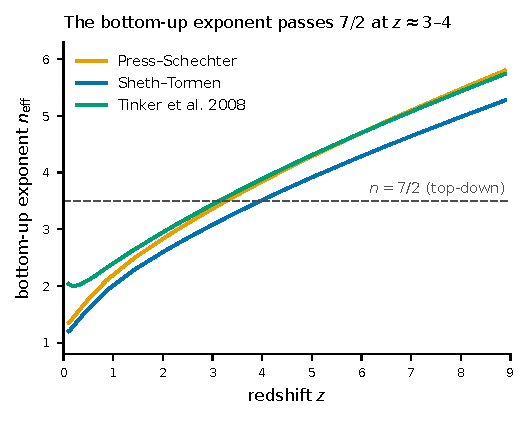
\includegraphics[width=0.62\textwidth]{figures/part2/fig_neff_bottomup.pdf}
\caption{Bottom-up exponent $n_{\rm eff}=d\ln[(dU/d\ln a)/f]/d\ln D$, with $U$ the virial kinetic energy summed over all halos, from three measured halo mass functions (Planck 2018 power spectrum; \texttt{colossus}; method of \texttt{docs/verification/scripts/\allowbreak{}verify\_bottom\_up\_exponent.py}). It equals the top-down $7/2$ at $z=3.3$ (Press--Schechter), 4.0 (Sheth--Tormen) and 3.2 (Tinker et al.\ 2008), and runs with redshift. \calc}\label{fig:neff_bottomup}
\end{figure}
Write the energy production rate as $\dot I\propto\rho_mD^nfH$ and the horizon accumulation as $dS_{\rm info}/dt=\dot I/(T_HA_H)$. In matter domination
$dS_{\rm info}/d\ln a\propto a^{n-9/2}$, and the form $\exp(1-1/a)$ requires $n-\tfrac92=-1$:
\begin{equation}n=\tfrac72\qquad\text{(top-down).}\end{equation}
\calc
The bottom-up rate is fixed with no choice left open. The factor $1/T_H$ is Landauer's (bits per unit energy), so $\dot I$ is a rate of energy; IAM's Law
with the virial partition fixes which energy --- the kinetic half of each bound structure, $K\simeq\tfrac12|W|\propto M^{5/3}(\Delta_c\rho_{\rm crit})^{1/3}$.
Summing $K$ over all halos with measured halo statistics (Planck 2018 power spectrum~\cite{Planck2018VI}; no mass threshold is needed, the sum converges at low mass) and
reading off $n_{\rm eff}=d\ln[(dU/d\ln a)/f]/d\ln D$:
\begin{center}\small\begin{tabular}{lcccc}\toprule
mass function & $n_{\rm eff}(z{=}4)$ & $n_{\rm eff}(z{=}2)$ & equals $7/2$ at & mean, $z=2.3$--$9$\\\midrule
Press--Schechter~\cite{PressSchechter1974} & 3.84 & 2.83 & $z=3.3$ & 4.26\\ Sheth--Tormen~\cite{ShethTormen1999} & 3.52 & 2.60 & $z=4.0$ & 3.89\\ Tinker et al.\ 2008~\cite{Tinker2008} & 3.89 & 2.95 & $z=3.2$ & 4.29\\\bottomrule
\end{tabular}\end{center}
The result is insensitive to the halo definition ($\pm0.03$) and to $\sigma_8$ between $0.77$ and $0.85$. The bottom-up exponent is not a constant: it
runs from about $5.5$ at $z=9$ to about $2$ at $z=1$, and passes through $7/2$ at $z\approx3$--$4$, averaging close to $4$ over the matter era. The two
directions meet at $7/2$ to within that running. \calc (Counting particles instead of energy, ``one bit per particle'', gives $n_{\rm eff}=\nu_{\min}^2-1$ for
Press--Schechter, with $\nu_{\min}$ set by an arbitrary mass threshold; it is inconsistent with the Landauer factor and is not used.) Open: whether
counting merger heating separately from the change in total halo kinetic energy flattens the running.
The top-down exponent and its dependence on the accumulation measure are derived in Appendix~\ref{app:der:exponent}. \openprob

\section{Light writes nothing in flight}
A photon travels a null geodesic, $d\tau=0$. It accumulates no proper time and makes no gravitational record in transit; its record is written where it
is absorbed, in matter. This is the sector split seen from the quantum side: matter on timelike worldlines writes, light does not, and so $\mu<1$ for
matter while $\Sigma=1$ for light.

\paragraph{Entanglement.} IAM's Law changes nothing in quantum mechanics. An entangled pair is one quantum state, and its correlations are those of that
state --- $|S|=2\sqrt2$ for an ideal source~\cite{Tsirelson1980} --- until an irreversible record is written. Photon pairs have been distributed over 1,200\,km by satellite
(Yin et al.\ 2017~\cite{Yin2017}); electron spins 1.3\,km apart have violated a Bell inequality without loopholes, entangled by interfering their spontaneously emitted
photons (Hensen et al.\ 2015~\cite{Hensen2015}). \observed\ Both are consistent with standard decoherence. The second shows a point the law makes precise: an emitted photon is not yet
a record, and its which-path information can still be erased by measuring it in a conjugate basis; the record is written, and the cost paid, where it is
absorbed.

\section{Massive superpositions}

\begin{figure}[htbp]\centering
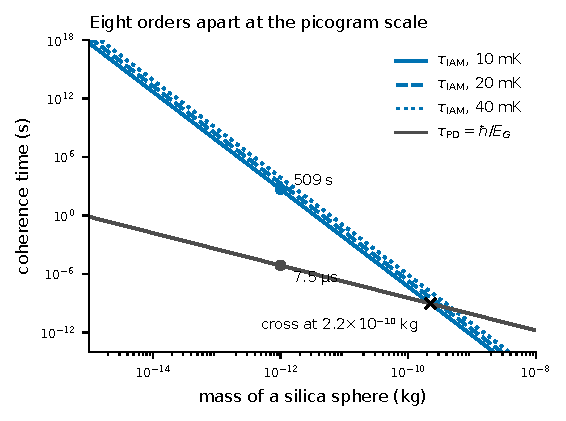
\includegraphics[width=0.62\textwidth]{figures/part2/fig_tau_mass.pdf}
\caption{Coherence time of a silica sphere ($\rho=2200$\,kg\,m$^{-3}$) in a spatial superposition: $\tau_{\rm IAM}=\hbar(k_BT)^2\ln2/E_G^3$ at 10, 20 and 40\,mK against $\tau_{\rm PD}=\hbar/E_G$, $E_G=Gm^2/R$. At $10^{-12}$\,kg and 10\,mK, 509\,s against 7.5\,$\mu$s; the two cross at $2.2\times10^{-10}$\,kg. The boundary capacity $k_BT/E_G$ behind $\tau_{\rm IAM}$ is assumed. \prediction\ \conjecture}\label{fig:tau_mass}
\end{figure}
For a massive object held in a spatial superposition, the gravitational self-energy $E_G\simeq Gm^2/R$ sets the scale of any gravitational channel.
Penrose and Di\'osi~\cite{Penrose1996,Diosi1987,Diosi1989} proposed a collapse time $\tau_{\rm PD}=\hbar/E_G$, independent of temperature. Applying IAM's Law at the superposition boundary,
with the boundary's capacity taken as $k_BT/E_G$, gives
\begin{equation}\tau_{\rm IAM}=\frac{\hbar\,(k_BT)^2\ln2}{E_G^3}\;\propto\;T^2m^{-5}\quad(\text{fixed density}),\qquad\tau_{\rm PD}\propto m^{-5/3}.\label{eq:qr_tauIAM}\end{equation}
For a $10^{-12}$\,kg silica sphere ($\rho=2200$\,kg\,m$^{-3}$) at 10\,mK: $\tau_{\rm IAM}=509$\,s, $\tau_{\rm PD}=7.5\,\mu$s; doubling the temperature
quadruples $\tau_{\rm IAM}$; the two times cross at $m\approx2.2\times10^{-10}$\,kg. The two proposals therefore differ by nearly eight orders of magnitude at
$10^{-12}$\,kg (a nanogram), and in their dependence on temperature. \calc A higher bath temperature lengthening a coherence time runs against every environmental channel,
which makes the $T^2$ law both the sharpest test and the most exposed claim.
The derivation is written out step by step, with the status of each premise, in Appendix~\ref{app:der:quantum}.

\paragraph{What is not yet derived.} The capacity $k_BT/E_G$ is assumed. The proposed time profile of the loss of coherence --- zero rate at first,
following the same $\exp(1-1/\eta)$ shape as $E(a)$ with $\eta=t/\tau_{\rm IAM}$ --- is carried over from the cosmology by analogy; the integral that
leads to it has a constant integrand and gives an exponential. Both need a derivation at the superposition boundary, the analogue of the surface density
on the horizon, before the profile can be used as a discriminator. \openprob Gravitational decoherence is irrelevant for present quantum processors: their
masses give $\tau_{\rm IAM}$ far beyond any practical time.

\section{Status}
Stands: IAM's Law gives Zurek's records their cost and their last surface \interp; decoherence of collapsed structure is instantaneous, so collapse
sets the writing rate \calc; priced by the law, measured halo statistics give a bottom-up exponent that passes through the $7/2$ that $E(a)$ requires at
$z\approx3$--$4$ and averages near 4 \calc; light writes nothing in flight; quantum mechanics, and with it every Bell test, is unchanged. Predicted:
$\tau_{\rm IAM}\propto T^2m^{-5}$ for massive superpositions. \prediction\ Open: the running of the bottom-up exponent; the boundary capacity and the
time profile of gravitational decoherence. \openprob
